%  article.tex (Version 1.00, released 1 October 2013)
%  LaTeX source file to demonstrate formatting for manuscripts 
%  to be submitted to SPIE journals
%  based on the class file spieman.cls, which requires 
%  the following standard packages:  times.sty, float.sty, 
%  ifthen.sty, cite.sty, color.sty, setspace.sty
%
%  Special instructions are included in this file after the
%  symbol %>>>>
%  Numerous commands are commented out, but included to show how
%  to effect various options, for example, to print page numbers, etc.
%  This LaTeX source file is composed for LaTeX2e.

%  The following commands have been added in the SPIE class 
%  file (spieman.cls) and may not be understood in other classes:
%  \affiliations{}, \sup{},\supit{}, \authorinfo{}, \keywords{},
%  \linkable and \video
%  The bibliography style file is called spiejour.bst 
%  This article.tex file needs the following image files:
%  mcr3b.eps
%  fig2.eps
%  satellite.eps

\documentclass[12pt]{spie}  %>>> 12pt font mandatory; use this for US letter paper 
%%\documentclass[a4paper,10pt]{spieman}  %>>> use this instead for A4 paper
%%\documentclass[nocompress,12pt]{spieman}  %>>> to avoid compression of citations
%% \addtolength{\voffset}{9mm}   %>>> moves text field down
%  The following command loads a graphics package to include images 
%  in the document. It may be necessary to specify a DVI driver option,
%  for example, [dvips], but that may be inappropriate for some LaTeX installations. 
\usepackage{amsmath}  %>>> for AMS math formatting, 
%  including bold Greek symbols
\usepackage[]{graphicx}
\usepackage{setspace}
\usepackage{tocloft}
\usepackage[]{times}


\title{Sample manuscript showing style and formatting specifications for SPIE journal papers} 

%>>>> The author is responsible for formatting the 
%  author list and their affiliations.  Use \\ to force linebreaks.
%  The correspondence between each author and his/her address
%  can be indicated with a superscript, 
%  which is easily obtained with \supscr{}.
%>>>> After the abstract, the author must include
%  a list of keywords and contact information for the corresponding author.

\author{First Author,\supscr{a} Second Author,\supscr{a} Third Author,\supscr{b} Fourth Author\supscr{a,b}}

\affiliation{\supscrsm{a}University Name, Faculty Group, Department, Street Address, City, Country, Postal Code\\
\supscrsm{b}Company Name, Street Address, City, Country, Postal Code}

%%%%%%%%%%%%%%%%%%%%%%%%%%%%%%%%%%%%%%%%%%%%%%%%%%%%%%%%%%%%% 
\renewcommand{\cftdotsep}{\cftnodots}
\cftpagenumbersoff{figure}
\cftpagenumbersoff{table} 
\begin{document} 
\maketitle 

%%%%%%%%%%%%%%%%%%%%%%%%%%%%%%%%%%%%%%%%%%%%%%%%%%%%%%%%%%%%% 
\begin{abstract}
This document shows the required format and appearance of a manuscript prepared for SPIE journals. It is prepared using LaTeX2e with the class file {\tt spieman.cls}. The abstract should consist of a single paragraph containing no more than 200 words. It should be a summary of the paper and not an introduction. Because the abstract may be used in abstracting and indexing databases, it should be self-contained (that is, no numerical references) and substantive in nature, presenting concisely the objectives, methodology used, results obtained, and their significance. A list of up to eight keywords should immediately follow, with the keywords separated by commas and ending with a period. The body of the manuscript should be double-spaced and fully justified.   
\end{abstract}

%>>>> Include a list of up to six keywords after the abstract
\keywords{optics, photonics, light, lasers, journal manuscripts, LaTeX template}

%>>>> Include contact information for corresponding author
{\noindent \footnotesize{\bf Address all correspondence to}: First author, University Name, Faculty Group, Department, Street Address, City, Country, Postal Code; Tel: +1 555-555-5555; Fax: +1 555-555-5556; E-mail:  \linkable{myemail@university.edu} }
%%%%%%%%%%%%%%%%%%%%%%%%%%%%%%%%%%%%%%%%%%%%%%%%%%%%%%%%%%%%%

\begin{spacing}{1}   % use double spacing for rest of manuscript

%%%%%%%%%%%%%%%%%%%%%%%%%%%%%%%%%%%%%%%%%%%%%%%%%%%%%%%%%%%%%
\section{Introduction}
\label{sect:intro}  % \label{} allows reference to this section
This document shows the required format and appearance of a manuscript prepared for SPIE journals. Formatting guidelines must be carefully followed. Authors are advised to print this sample manuscript and use it as a reference while preparing their own paper, to ensure all guidelines are met.

%%-----------------------------------------------------------
\subsection{Use of This Document}

This document is prepared using LaTeX2e\cite{Lamport94,Goossens97} with the class file {\ttfamily spieman.cls}.  The LaTeX source file used to create this document is {\ttfamily article.tex}, which contains important formatting information embedded in it. Authors may use it as a template to create their own manuscript. While LaTeX properly handles most formatting issues, the author may occasionally need to intervene to obtain a satisfactorily  formatted manuscript.

%%-----------------------------------------------------------
\subsection{English}

Authors are strongly encouraged to follow the principles of sound technical writing, as found in Refs.~\citenum{Alred03} and \citenum{Perelman97}, for example. In addition, good English usage is essential. Authors whose native language is not English may wish to collaborate with a colleague whose English skills are more advanced. Alternatively, you may wish to have your manuscript professionally edited prior to submission by Editage, our recommended independent editorial service: \linkable{http://spie.org/EnglishEditing}. SPIE authors will receive a 10\% discount off their services. A spell checker can be helpful to discover misspelled words, but authors should also proofread their papers carefully prior to submission. Manuscripts that do not meet acceptable English standards or lack clarity may be rejected.

%%-----------------------------------------------------------
\subsection{Page Setup and Fonts}

All text and figures, including footnotes, must fit inside a text area 6.5 in.\ wide by 9 in.\ high (16.51 by 22.86 cm). Manuscripts must be formatted for US letter paper, on which the margins should be 1.0 in.\ (2.54 cm) on the top, 1 in.\ on the bottom, and 1 in\ on the left and right. 

The Times New Roman font is used throughout the manuscript, in the sizes and styles shown in Table~\ref{tab:fonts}. If this font is not available, use a similar serif font. The manuscript should not contain headers or footers. Pages should be numbered.

%% Use of [h] in following command forces table to appear "here", instead of a top or bottom of page, which is generally preferred.
\begin{table}[h]
\caption{Fonts sizes and styles.} 
\label{tab:fonts}
\begin{center}       
\begin{tabular}{|l|l|} %% this creates two columns
%% |l|l| to left justify each column entry
%% |c|c| to center each column entry
%% use of \rule[]{}{} below opens up each row
\hline
\rule[-1ex]{0pt}{3.5ex}  Document entity & Brief description  \\
\hline\hline
\rule[-1ex]{0pt}{3.5ex}  Article title & 16 pt., bold, left justified  \\
\hline
\rule[-1ex]{0pt}{3.5ex}  Author names & 12 pt., bold, left justified   \\
\hline
\rule[-1ex]{0pt}{3.5ex}  Author affiliations & 10 pt., left justified   \\
\hline
\rule[-1ex]{0pt}{3.5ex}  Abstract & 10 pt.  \\
\hline
\rule[-1ex]{0pt}{3.5ex}  Keywords & 10 pt.  \\
\hline
\rule[-1ex]{0pt}{3.5ex}  Section heading & 12 pt., bold, left justified  \\
\hline
\rule[-1ex]{0pt}{3.5ex}  Subsection heading & 12 pt., italic, left justified  \\
\hline
\rule[-1ex]{0pt}{3.5ex}  Sub-subsection heading & 11 pt., italic, left justified  \\
\hline
\rule[-1ex]{0pt}{3.5ex}  Normal text & 12 pt. \\
\hline
\rule[-1ex]{0pt}{3.5ex}  Figure and table captions &  10 pt. \\
\hline 
\end{tabular}
\end{center}
\end{table} 

%%%%%%%%%%%%%%%%%%%%%%%%%%%%%%%%%%%%%%%%%%%%%%%%%%%%%%%%%%%%%
\section{Parts of Manuscript} 

This section describes the normal structure of a manuscript and how each part should be handled. The appropriate vertical spacing between various parts of this document is achieved in LaTeX through the proper use of defined constructs, such as \verb|\section{}|. 

%%-----------------------------------------------------------
\subsection{Title and Author Information} 
\label{sect:title}
The article title appears left justified at the top of the first page. The title font is 16 pt., bold. The rules for capitalizing the title are the same as for sentences; only the first word, proper nouns, and acronyms should be capitalized. Do not begin titles with articles (for example, a, an, the) or prepositions (for example, on, by, etc.). The word �novel� should not appear in the title, as publication will imply novelty. Avoid the use of acronyms in the title, unless they are widely understood. Appendix A contains more about acronyms.

The list of authors immediately follows the title, 18 points below. The font is 12 pt., bold and the author names are left justified. The author affiliations and addresses follow the names, in 10-pt., normal font and left justified. For multiple affiliations, each affiliation should appear on a separate line. Superscript letters (a, b, c, etc.) should be used to associate multiple authors with their respective affiliations. Corresponding author should be listed below the Keywords, following the line ``Address all correspondence to:"; include mailing address, telephone, fax, and E-mail address.

%%-----------------------------------------------------------
\subsection{Abstract} 
The abstract should be a concise summary of the paper. Because the abstract may be used in abstracting journals, it should be self-contained (that is, no numerical references) and substantive in nature, presenting concisely the objectives, methodology used, results obtained, and their significance. It should not exceed 200 words. For further guidelines, please read the brief article titled ``How to Write an Abstract (PDF)," \\(\linkable{http://spie.org/Documents/Publications/How to Write an Abstract.pdf}) by Philip Koopman. (Courtesy of Philip Koopman, Carnegie Mellon University.) Note the underlined link must be written on a single line in order for the link to function. Thus, a break in the line, created with {\verb+\\+} is required before the link or the preceding text should be editted to gracefully place the link on a single line. This type of adjustment is best done at end of the manuscript-preparation process.

%%-----------------------------------------------------------
\subsection{Keywords} 
Up to eight keywords should be specified. 

%%-----------------------------------------------------------
\subsection{Body of Paper} 
The body of the paper consists of numbered sections that present the main findings. These sections should be organized to best present the material.

To provide transition elements in your paper, it is important to refer back (or forward) to specific sections. Such references are made by indicating the section number, for example, ``In Sec.\ 2 we showed..." or ``Section 2.1 contained a description..." If the word Section, Reference, Equation, or Figure starts a sentence, it is spelled out. When occurring in the middle of a sentence, these words are abbreviated Sect., Ref., Eq., and Fig. 

At the first occurrence of an acronym, spell it out followed by the acronym in parentheses, for example, charge-coupled diode (CCD).

%%-----------------------------------------------------------
\subsection{Footnotes} 
Use textual footnotes only when necessary to present important documentary or explanatory material whose inclusion in the text would be distracting.\footnote{Example of a footnote.} Due to problems with HTML display, use of footnotes should be avoided. If absolutely necessary, the footnote mark must come at the end of a sentence. To insert a footnote, use the {\verb|\footnote{}|} command.

%%-----------------------------------------------------------
\subsection{Appendices} 
SPIE journals do not accept supplementary materials. However, it is acceptable to include an Appendix when necessary,  details such as derivations of equations, proofs of theorems, and details of algorithms. Equations and figures appearing in appendices should continue sequential numbering from earlier in the paper.

%%-----------------------------------------------------------
\subsection{Acknowledgments} 
In the acknowledgments section, which appears just before the references, the authors may credit others for their guidance or help. Also, funding sources or sponsorship information may be stated. The acknowledgments section does not have a section number.

%%-----------------------------------------------------------
\subsection{References} 
The References section lists books, articles, and reports that are cited in the paper. This section does not have a section number. The references are numbered in the order in which they are cited. Examples of the format to be followed are given at the end of this document.

The reference list at the end of this document is created using BibTeX, which looks through the file {\ttfamily report.bib} for the entries cited in the LaTeX source file.  The format of the reference list is determined by the bibliography style file {\ttfamily spiejour.bst}, as specified in the \\ \verb|\bibliographystyle{spiejour}| command.  Alternatively, the references may be directly formatted in the LaTeX source file.

For books\cite{Lamport94,Alred03,Goossens97} the listing includes the list of authors (initials plus last name), book title (in italics), page or chapter numbers, publisher, city, and year of publication.  Journal-article references \cite{Metropolis53,Harris06} include the author list, title of the article (in quotes), journal name (in italics, properly abbreviated), volume number (in bold), inclusive page numbers or citation identifier, and year.  A reference to a proceedings paper or a chapter in an edited book\cite{Gull89a} includes the author list, title of the article (in quotes), conference name (in italics), editors (if appropriate), volume title (in italics), volume number if applicable (in bold), inclusive page numbers, publisher, city, and year.  References to an article in the SPIE Proceedings may include the conference name, as shown in Ref.~\citenum{Hanson93c}.

The references are numbered in the order of their first citation. Citations to the references are made using superscripts, as demonstrated in the preceding paragraph. One may also directly refer to a reference within the text, for example, ``as shown in Ref.~\citenum{Metropolis53} ..."  Two or more references should be separated by a comma with no space between them. Multiple sequential references should be displayed with a dash between the first and last numbers \cite{Alred03,Perelman97,Lamport94,Goossens97,Metropolis53}. 

%%---------------------------
\subsubsection{Reference linking and DOIs} 
A Digital Object Identifier (DOI) is a unique alphanumeric string assigned to a digital object, such as a journal article or a book chapter, that provides a persistent link to its location on the internet. The use of DOIs allows readers to easily access cited articles. Authors should include the DOI at the end of each reference in brackets, if a DOI is available. See examples at the end of this manuscript. A free DOI lookup service is available from CrossRef at \\\linkable{http://www.crossref.org/freeTextQuery/}. The inclusion of DOIs will facilitate reference linking and is highly recommended. 

In the present LaTeX template, the author needs to add the DOI reference by including it in a ``note" in the bibliography file, as shown in the file {\verb+report.bib+}, for example, \\ {\verb+note = "[doi:10.1117/12.154577]"+}. The DOI may be used by the reader to locate that document with the link: {\verb+http://dx.doi.org10.1117/12.154577+}. 

%%-----------------------------------------------------------
\subsection{Biographies} 
A brief professional biography not to exceed 75 words may be provided for each author, if available. Biographies should be placed at the end of the paper, after the references. Personal information such as hobbies or birthplace/birthdate should not be included. Author photographs are not published.

%%%%%%%%%%%%%%%%%%%%%%%%%%%%%%%%%%%%%%%%%%%%%%%%%%%%%%%%%%%%%
\section{Section Formatting} \label{sect:sections}

In LaTeX, a new section is created with the \verb|\section{}| command, which automatically numbers the sections. Sections will be numbered sequentially, starting with the first section after the abstract, except for the acknowledgments and references. (Note that numbering of section headings is not required, but the numbering must be consistent if used.) All section headings should be left justified.

Main section headings are in 12-pt., bold font, left-justified and in title case, where important words are capitalized.

Paragraphs that immediately follow a section heading are leading paragraphs and should not be indented, according to standard publishing style. The same goes for leading paragraphs of subsections and sub-subsections. Subsequent paragraphs are standard paragraphs, with 0.2-in (5 mm) indentation. There is no additional space between paragraphs. In LaTeX, paragraphs are separated by blank lines in the source file. Indentation of the first line of a paragraph may be avoided by starting it with \verb|\noindent|.

%%-----------------------------------------------------------
\subsection{Subsection Headings} 
All important words in a subsection (level 1) header are capitalized. Subsection numbers consist of the section number, followed by a period, and the subsection number within that section, without a period at the end. The heading is left justified and its font is 12 pt., italic.

%%-----------
\subsubsection{Sub-subsection headings} 
The first word of a sub-subsection is capitalized. The rest of the text is not capitalized, except for proper names and acronyms (the latter should only be used if well known). The heading is left justified and its font is 11 pt., italic. 

%%%%%%%%%%%%%%%%%%%%%%%%%%%%%%%%%%%%%%%%%%%%%%%%%%%%%%%%%%%%%
\section{Figures and Tables} 

%%-----------------------------------------------------------
\subsection{Figures} 

Figures are numbered in the order in which they are called out in the text. They should appear in the document in numerical order and as close as possible to their first reference in the text. It may be necessary to move figures or tables around to enhance readability. LaTeX will attempt to place figures at the top or bottom of a page in which they are first referenced.

Figures, along with their captions, should be separated from the main text by  0.2 in.\ or 5 mm and centered. Figure captions are centered below the figure or graph. Figure captions start with the abbreviation ``Fig" in front of the figure number, followed by a period, and the text in 10-pt. font. See Fig.~\ref{fig:example} for an example.

%%  Use following command to specify that graphics file is in 
%%  a directory other than this LaTeX source file.
%%  Note use of / to separate subdirectories, for UNIX and Windows OS.
%-------------
   \begin{figure}
   \begin{center}
   \begin{tabular}{c}
   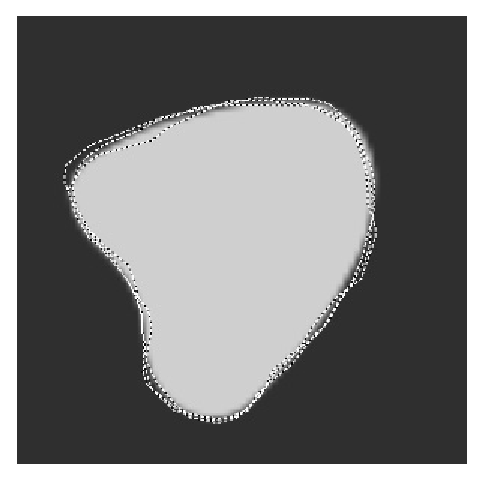
\includegraphics[height=5.5cm]{mcr3b.eps}
   \end{tabular}
   \end{center}
   \caption 
   { \label{fig:example} %>> use \label inside caption to get Fig. number with \ref{}
Example of a figure caption. } 
   \end{figure} 
%-------------
Authors may wish to create figures consisting of two or more images, in which case, they should be neatly arranged in a rectangular array.  In no case, should the article's text be wrapped around a figure. Figure~\ref{fig:example2} shows two side-by-side images. When a figure contains more than one image, the author must submit them as a single image file. Further details about figure formatting can be found at \linkable{http://spie.org/x85020.xml
\#Components}. 

%------------- 
   \begin{figure}
   \begin{center}
   \begin{tabular}{c}
   
\includegraphics[height=5.5cm]{fig2.eps}  % fig2 includes two images 
     \\
     (a) \hspace{5.1cm} (b)
   \end{tabular}
   \end{center}
   \caption 
   { \label{fig:example2} %>> use \label inside caption to get Fig. number with \ref{}
Example of a figure containing multiple images: (a) sun and (b) blob. Figures containing multiple images must be submitted to SPIE as a single image file.} 
   \end{figure} 

%-------------%%-----------------------------------------------------------
\subsection{Tables} 
Tables are numbered in the order in which they are referenced. They should appear in the document in numerical order and as close as possible to their first reference in the text. It is preferable to have tables appear at the top or bottom of the page, if possible. Table captions are handled identically to those for figures, except that they appear above the table. See Table~\ref{tab:fonts} for an example.
%%-----------------------------------------------------------

\subsection{Multimedia} 
Please refer to the multimedia guidelines at \linkable{http://spie.org/x85020.xml\#Multimedia} for specific submission guidelines and requirements. The following types of multimedia files are accepted: QuickTime Non-Streaming video (.qt or .mov), MPEG (.mpg or .mp4). The recommended maximum size for each multimedia file is 10-12 MB. Authors must insert a representative �still� image from the video file in the manuscript as a �figure.� This still image will be linked by the publisher to the actual video file, as will the caption label. Multimedia files are treated in the same manner as figures and they will be numbered sequentially with normal figures. Otherwise  The multimedia file type should be included in parentheses at the end of the figure caption, along with the file size. See Video \ref{vid:satellite} for an example.

%-------------
   \begin{video}
   \begin{center}
   {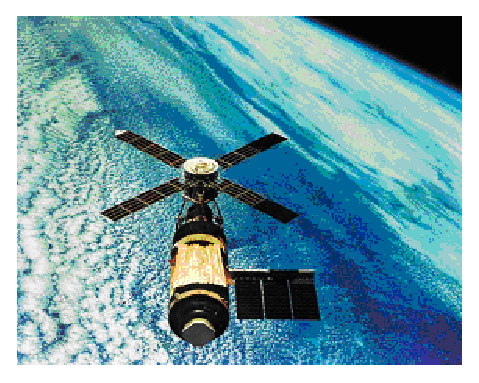
\includegraphics[height=5cm]{satellite.eps}}
   \\
   \end{center}
   \caption{\label{vid:satellite} Example of a multimedia still image (MPEG, 2.5 MB).}
   \end{video} 
%-------------

 
%%%%%%%%%%%%%%%%%%%%%%%%%%%%%%%%%%%%%%%%%%%%%%%%%%%%
\appendix    %>>>> this command starts appendixes
%%%%%%%%%%%%%%%%%%%%%%%%%%%%%%%%%%%%%%%%%%%%%%%%%%%%
\section{Miscellaneous Formatting Details} \label{sect:misc}

At times it may be desired, for formatting reasons, to break a line without starting a new paragraph. In a LaTeX source file, a linebreak is created with \verb|\\|.

%%-----------------------------------------------
\subsection{Formatting Equations} 
Equations may appear inline with the text, if they are simple, short, and not of major importance; for example, $\beta = b/r$.  Important equations appear on their own line.  Such equations are centered.  For example, ``The expression for the field of view is
	\begin{equation}
	\label{eq:fov}
2 a = \frac{(b + 1)}{3c} \, ,
	\end{equation}
where $a$ is the ..."  Principal equations are numbered, with the equation number placed within parentheses and right justified.  

Equations are considered to be part of a sentence and should be punctuated accordingly. In the above example, a comma appears after the equation because the next line is a subordinate clause. If the equation ends the sentence, a period should follow the equation. The line following an equation should not be indented unless it is meant to start a new paragraph. Indentation after an equation is avoided in LaTeX by not leaving a blank line between the equation and the subsequent text.

References to equations include the equation number in parentheses, for example, ``Equation~(\ref{eq:fov}) shows ..." or ``Combining Eqs.~(2) and (3), we obtain..." Note that the word ``Equation" is spelled out if it begins a sentence, but is abbreviated as ``Eq." otherwise. Using a tilde in the LaTeX source file between two characters avoids unwanted line breaks, for example between ``Eq." and the following equation number..

%%-----------------------------------------------------------
\subsection{Formatting Theorems} 

To include theorems in a formal way, the theorem identification should appear in a 10-point, bold font, left justified, and followed by a period.  The text of the theorem continues on the same line in normal, 10-pt. font, achieved in LaTeX using \verb|\footnotesize|.  For example, 

\vspace{2ex}\noindent{\footnotesize{\bf Theorem 1.} For any unbiased estimator...}

%%%%%%%%%%%%%%%%%%%%%%%%%%%%%%%%%%%%%%%%%%%%%%%%%%%%
\section{Some LaTeX Guidance} \label{sect:latex}

To work properly, the LaTeX style file {\ttfamily spieman.cls} used to create this document requires following LaTeX packages:
{\ttfamily times.sty}, {\ttfamily float.sty}, {\ttfamily ifthen.sty}, {\ttfamily setspace.sty}, \\{\ttfamily cite.sty} (version 4.01 or later), and {\ttfamily color.sty}. If you do not have them in your LaTeX environment, see your system manager, or download them from \linkable{http://www.ctan.org}. 

The author is required to make sure his or her manuscript is properly formatted. LaTeX sometimes needs some help to avoid making gross formatting blunders. The source file for this document provides examples of how to cope with some of LaTeX's shortcomings.

%%-----------------------------------------------------------
\subsection{Margins and PostScript Fonts}
 
Manuscripts submitted for SPIE journals as Portable Document Format (PDF) files must be formatted for US-letter-size paper and have the correct margins. The output of the LaTeX utility is a file with the extension DVI (for Device Independent), which encodes the formatted document. 

One may directly create a PDF file from the DVI file with the LaTeX utility {\ttfamily dvipdfm}, for example. No options are necessary. Appealing aspects of this utility are that Acrobat Distiller is not needed, and Type 1 PostScript fonts are automatically included in the resulting PDF file.  Furthermore, {\ttfamily dvipdfm} allows one to directly incorporate images in JPEG, PNG, and PDF formats, and not just EPS, which is normally used with LaTeX. 

Alternatively, with an application such as Adobe Acrobat, PDF files can be created from PostScript (PS) files, which can be produced by DVIPS. In most cases, the following DVIPS options should be invoked.

An important DVIPS option specifies the incorporation of (scalable) PostScript Type 1 fonts in its output PS file. This feature is important for obtaining a subsequent PDF file that will be clearly displayed on a computer monitor by Adobe Acrobat Reader.  The option ``{\ttfamily -P pdf}" makes DVIPS include these fonts in its output PS file.

LaTeX margins are related to the document's paper size. The paper size is set at two separate places in the process of creating a PS file. The first place is in {\ttfamily latex}. 
The second place is in the application DVIPS. DVIPS has its own default paper size, which can be overridden with the option ``{\ttfamily -t letter}" or ``{\ttfamily -t a4}".  
If the foregoing steps do not produce the correct top margin, you can move the text lower on the page (by 9 mm) with the command \verb|\addtolength{\voffset}{9mm}|, placed right after the \verb|\documentclass| command.

The {\ttfamily times.sty} package produces a bug in the handling certain combinations of letters; for example, `fi' is interpretted as a British pound symbol. Use the option ``{\ttfamily -G0}" ( capital G and zero) to avoid this problem.

To summarize, the following DVIPS options are recommended when making the PS file: ``{\ttfamily -t letter -P pdf -G0}".

%%-----------------------------------------------------------
\subsection{Bold Math Symbols} 

The math package from the American Mathematical Society allows one to easily produce bold math symbols, well beyond what is available in LaTeX. It also provides many useful capabilities for creating elaborate mathematical expressions. You need to load the AMS math package near the top of the LaTeX source file, right after the \verb+\documentclass+ command:\\[1ex]
\verb+\usepackage[]{amsmath}+ \\[1ex]
Then for bold math symbols, use \verb+\boldsymbol+; for example, 
\verb+$\boldsymbol{\pi}$+ 
yields a bold pi.  You can make it easier to use by defining a shorthand command:\\[1ex]
\verb+\newcommand{\bm}[1]{\boldsymbol{#1}}+ \\[1ex]
and then using it like so \verb+$\bm{\pi}$+.

Not all math symbols are available in bold.  In a pinch, you can use \verb+\pmb+ ("poor man's bold"), which is defined in \verb+amsmath+. This command approximates a bold character with a superposition of several, slightly displaced unbold characters.

If you want a Greek symbol in the article title, it should be both larger and bold. The easiest thing is to load the AMS math package as described above. 
Then, in the title, use something like:\\[1ex]
\verb+\title{Estimation of {$\boldsymbol\alpha$} by a Monte Carlo + \linebreak\verb+technique}+ \\[1ex]
Note that the command to create the alpha character is enclosed within braces to form a self-contained environment. 

%%-----------------------------------------------------------
\subsection{Uppercase Letters and Special Symbols in BibTex and LaTeX} 

BibTeX tries to enforce standard publishing rules regarding article titles and authors' names; it sometimes changes uppercase letters to lower case. LaTeX does the same thing for the article title. BibTeX also has trouble with umlauts, generally created in LaTeX with \verb+\"{o}+, because it is looking for the \verb+"+ to end the input line. 

The general rule for overriding LaTeX's and BibTex's reinterpretation of your input text is to put the items you wish to be unchanged within braces \verb!{}!. Thus, to obtain an umlaut in an author's name or in an article title, or to force an uppercase letter, do something like the following: \\[1ex]
\verb+ @article{Kaczmarz37,+ \\ 
\verb+ author = "S. Kaczmarz",+ \\ 
\verb+ title  = "Angen{\"{a}}hrte {A}ufl{\"{o}}sung von {S}ystemen + \linebreak\verb+linearer {G}leichungen",+ \\ 
\verb+ journal= "Bull. Acad. Polon. Sci. Lett.",+ \\ 
\verb+ volume = "A35",+ \\ 
\verb+ pages  = "355-357",+ \\	
\verb+ year   = "1937"	} + \\[1ex]
This example shows the treatment for both umlauts and uppercase letters.
%%%%%%%%%%%%%%%%%%%%%%%%%%%%%%%%%%%%%%%%%%%%%%%%%%%%%%%%%%%%%
\acknowledgments 
This unnumbered section is used to identify those who have aided the authors in understanding or accomplishing the work presented and to acknowledge sources of funding.  

%%%%%%%%%%%%%%%%%%%%%%%%%%%%%%%%%%%%%%%%%%%%%%%%%%%%%%%%%%%%%
%%%%% References %%%%%

\bibliography{report}   %>>>> bibliography data in report.bib
\bibliographystyle{spiejour}   %>>>> makes bibtex use spiejour.bst

%%%%%%%%%%%%%%%%%%%%%%%%%%%%%%%%%%%%%%%%%%%%%%%%%%%%%%%%%%%%%
%%%%% Biographies of authors %%%%%

\vspace{2ex}\noindent{\bf First Author} is an assistant professor at the University of Optical Engineering. He received his BS and MS degrees in physics from the University of Optics in 1985 and 1987, respectively, and his PhD degree in optics from the Institute of Technology in 1991.  He is the author of more than 50 journal papers and has written three book chapters. His current research interests include optical interconnects, holography, and optoelectronic systems. He is a member of SPIE.

\vspace{1ex}
\noindent Biographies and photographs of the other authors are not available.

\listoffigures
\listoftables

\end{spacing}
\end{document} 
